\begin{figure}[htpb]
	\centering\capstart{}
	\subfloat[Dirac delta function]
	{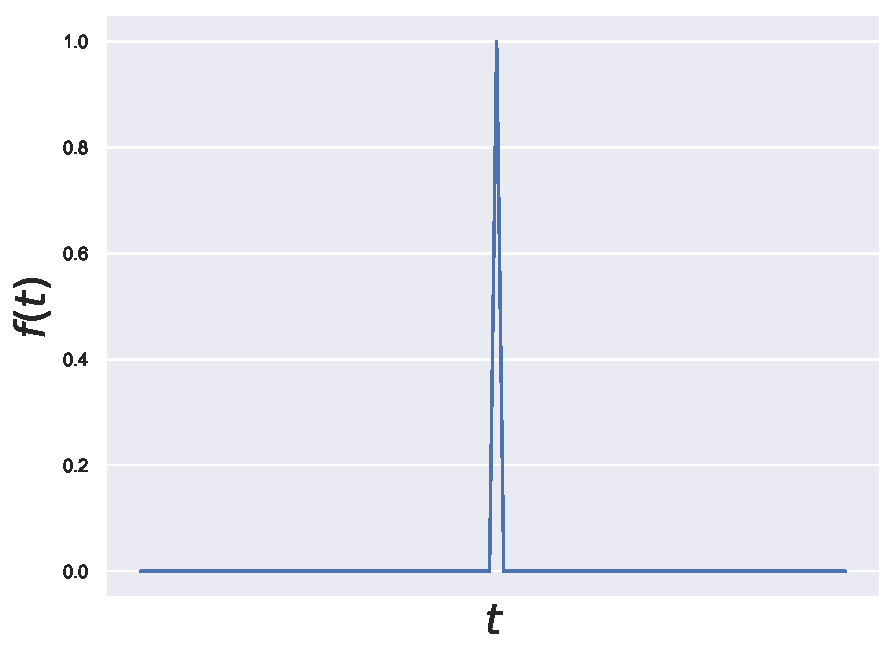
\includegraphics[width=.49\textwidth]{dirac_impulse.pdf}}
	\hfill
	\subfloat[After a Fourier transform]
	{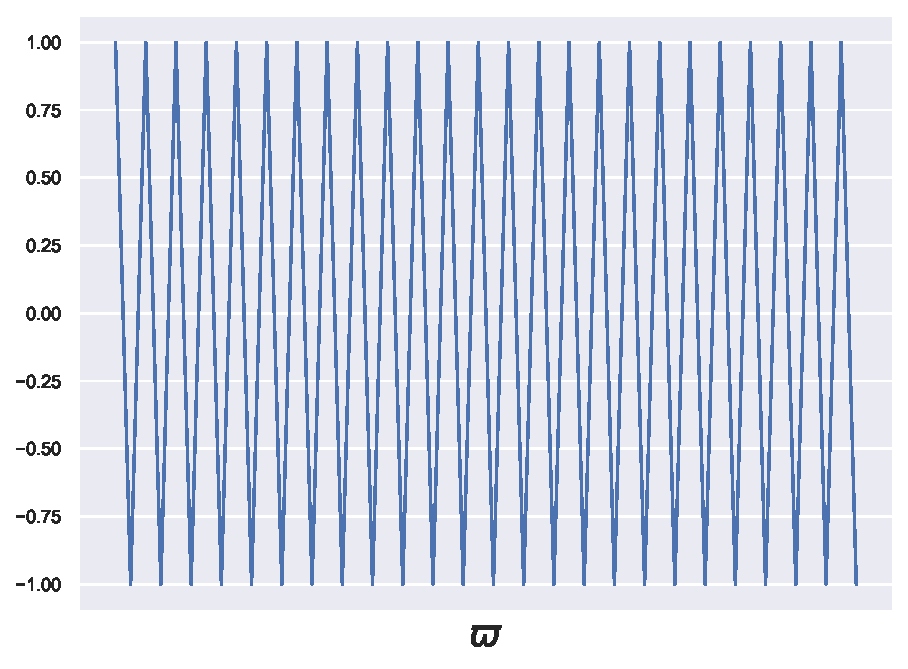
\includegraphics[width=.49\textwidth]{dirac_fft.pdf}}
	\caption[
		A Dirac delta function and the result of a Fourier transform
	]{
		A visual demonstration of the problem with the Fourier transform.
		Panel (a) presents a Dirac delta in the time-domain; which is well-localised in time, as expected.
		The result of a Fourier transform is shown in panel (b), which now consists of all possible frequencies.
		This phenomenon occurs due to the Heisenberg uncertainty principle.
	}\label{fig:chapter2_dirac_fourier}
\end{figure}
